\documentclass[a4paper,12pt]{scrartcl}
  \usepackage[utf8]{inputenc}
  \usepackage[T1]{fontenc}
  \usepackage{gfsartemisia-euler}
  \usepackage[brazil]{babel}
  \usepackage{paralist}
  \usepackage{amsmath}
  \usepackage{amssymb}
  \usepackage{geometry}
  \usepackage{hyperref}
  \usepackage[squaren]{SIunits}
  \usepackage{indentfirst}
  \usepackage{graphicx}
  \usepackage[font=small,format=plain]{caption}
  \usepackage{icomma}
  
  
  \title{Proposta de atividade 1:}
  \subtitle{o teorema fundamental do Cálculo}
  \author{R. S. Morais, S. N. Dezidério, I. R. Pagnossin}

  \hyphenation{pro-ble-ma pri-mi-ti-va}
  
\begin{document}

  \setlength\parindent{2em}

  \maketitle

  \begin{abstract}
    Este trabalho apresenta uma proposta de atividade de aprendizagem que utiliza o recurso educacional interativo ``Integral de Riemann'' (disponível \href{http://cepa-usp.github.io/AI-0170/}{aqui}) para abordar o \emph{teorema fundamental do Cálculo}: utilizamos o software para construir uma soma de Riemann arbitrária, com o intuito de aproximar a área sob o gráfico de uma função afim $f$ no intervalo $[a,b]$ e comparamos o resultado com a área exata, que pode ser obtida geometricamente. Finalmente, utilizamos a anti-derivada $F$ para evidenciar a equivalência desses resultados com $F(b) - F(a)$.
    
    Como o software oferece bastante flexibilidade na construção das somas de Riemann, podemos aproximar a área sob $f$ utilizando uma quantidade finita de elementos de área, fundamentado no \emph{teorema do valor médio} para integrais (que não é abordado explicitamente). Por isso, propomos uma atividade com foco na participação dos alunos, baseando todo o processo em conhecimentos prévios deles.
    
    Para mais instruções sobre como utilizar o recurso educacional, veja \href{http://www.youtube.com/watch?v=PJlPleMYuG4&t=22}{este tutorial}.
  \end{abstract}
  
  \section*{Parte 1}
  
    Nesta primeira parte da atividade, construiremos uma soma de Riemann da \emph{função afim} $f(x) = 2x + 1$, cuja área sob ela pode ser calculada com base em argumentos geométricos (áreas do triângulo, do retângulo e do trapézio), conhecidos do aluno. Deste modo e utilizando implicitamente o \emph{teorema do valor médio} para integrais, poderemos construir uma soma de Riemann com poucos elementos de área e mostrar como o resultado da soma equipara-se ao cálculo analítico da integral definida, evidenciando assim o \emph{teorema fundamental do Cálculo}.
    
    Neste processo, é importante que os alunos sejam estimulados a participar, propondo o próximo passo na solução do problema que queremos resolver, a saber: encontrar o valor da área da região delimiteada por $x = a$, $x = b$, $y = 0 $ e $y = f(x)$ (a ``área sob $f$'').
  
    \subsection*{Objetivos específicos}
  
    Ao final desta atividade, espera-se que os alunos saibam:
    \begin{compactitem}
      \item explicar o significado o termo \emph{soma de Riemann}.
      \item explicar a importância do \emph{teorema fundamental do Cálculo}.
      \item explicar a relação entre os dois conceitos acima.
    \end{compactitem}
  
    \subsection*{Roteiro}
  
    \newcounter{steps}
    \begin{list}{\arabic{steps}.}{
	\setlength\leftmargin{0cm}%
	\setlength\itemindent\parindent%
	\setlength\listparindent{\parindent}%
        \setlength\labelwidth{1.3em}%
        \setlength\labelsep{0.7em}%        
        \refstepcounter{steps}%
        \usecounter{steps}%
    }
  
      \item Utilize o recurso educacional para desenhar o gráfico da \emph{função afim} $f(x) = 2x + 1$. Para isso, escolha esta função na tela 1 do software, no grupo ``funções polinomiais'', e avance para a tela 2 (figura~\ref{fig:f}).
            
      \begin{figure}
	\begin{minipage}[t]{0.49\textwidth}
	  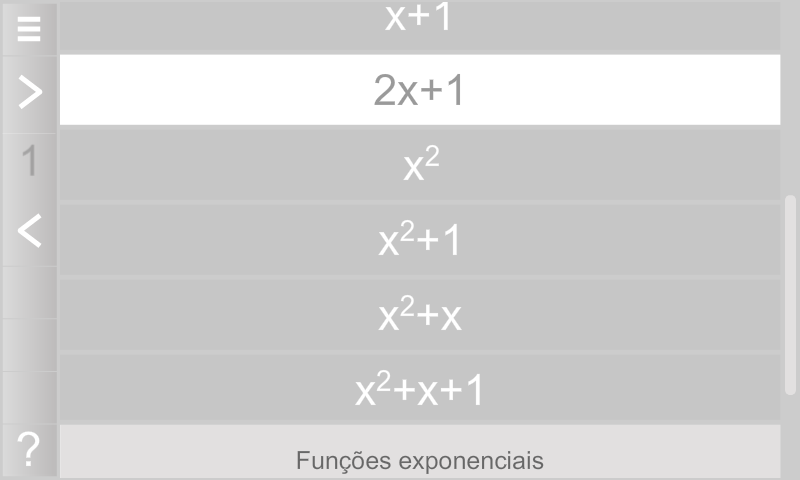
\includegraphics[width=\textwidth]{f.png}	  
	\end{minipage}
	\hfill
	\begin{minipage}[t]{0.49\textwidth}
	  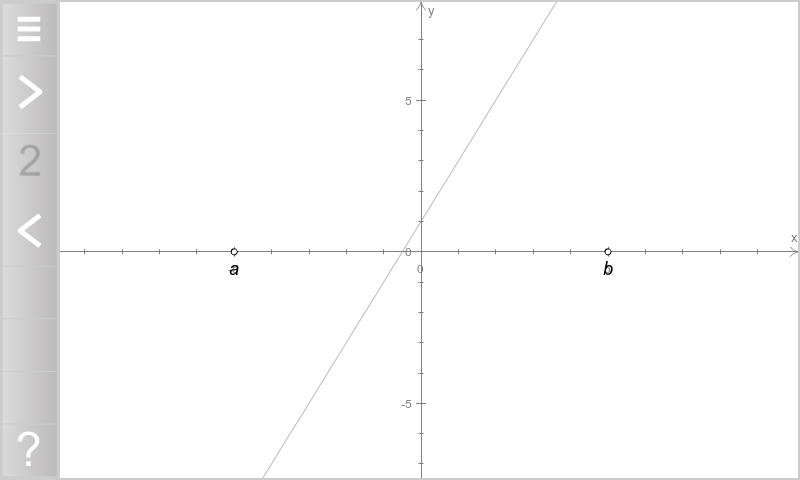
\includegraphics[width=\textwidth]{grafico-f.png}
	\end{minipage}
	\caption{selecione a função $f(x) = 2x + 1$ na tela 1 (à esquerda) e avance para a tela 2, onde seu gráfico será automaticamente desenhado (à direita).}
	\label{fig:f}
      \end{figure}
      
      \item Escolha o intervalo de integração $[a,b]=[0,3]$: na tela 2, arraste o ponto $a$ para a abscissa $x = 0$ e o ponto $b$, para $x = 3$. Feito isso, avance para a tela 3.
      
      \item Escolha a opção ``soma personalizada'' na tela 3, o que lhe dará mais flexibilidade para construir a soma de Riemann. Avance para a tela 4.
      
      \item \label{step:area} Na tela 4 haverá, inicialmente, apenas os limites inferior ($a$) e superior ($b$) de integração. Questione os alunos sobre como calcular a área sob o gráfico de $f(x) = 2x + 1$ no intervalo escolhido. Espera-se que eles proponham utilizar a fórmula da área do trapézio de altura $b - a = 3$ e bases $f(a) = 1$ e $f(b) = 7$. Neste caso a área será
      \begin{equation*}
	\text{Área sob $f$} = \frac{1}{2}\left[f(a) + f(b)\right](b - a).
      \end{equation*}
      
      Alternativamente, os alunos podem sugerir somar a área do retângulo de lados $b - a$ e $f(a)$ com a área do triângulo de base $b - a$ e altura $f(b) - f(a)$. Neste caso, a área será dada por
      \begin{equation*}
       \text{Área sob $f$} = (b - a)f(a) + \frac{1}{2}(b - a)\left[f(b) - f(a)\right].
      \end{equation*}
      
      Obviamente as duas expressões resultam no mesmo valor: 12.

      \item Após determinar a área sob $f$ no intervalo $[a,b]$, questionar os alunos sobre como obter um valor \emph{aproximado} dessa área utilizando apenas retângulos. Espera-se que eles sugiram a inserção de vários retângulos abaixo do gráfico de $f$ (soma inferior) ou acima dele (soma superior), no intervalo de integração.
      
      Provavelmente os alunos questionarão o porquê dessa necessidade, haja vista que as fórmulas da Geometria Euclidiana Plana resolvem o problema.
      Este é um bom momento para propor que eles pensem em como \emph{aproxiar} a área sob a função $x^2$ no mesmo intervalo de integração.
    
      \item Após a discussão acima, ainda na tela 4, crie uma partição do intervalo $[a,b]$. Ou seja, escolha um conjunto de pontos sobre o eixo das abscissas que, juntamente com os pontos $a$ e $b$, dividem o intervalo de integração em $n = 5$ (ou mais) subintervalos. 
      
      Para criar um ponto da partição, clique com o mouse sobre o eixo das abscissas, na posição $x_i \in ]a,b[$ em que se quer criar o ponto. Em seguida, pressione o botão $+$ (mais), na barra de ferramentas, à esquerda da tela. Alternativamente, \emph{posicione} o mouse sobre o ponto desejado e pressione a tecla \textit{p}. Para remover este ponto, clique com o mouse sobre ele para selecioná-lo e pressione o botão $-$ (menos), ou pressione ``delete'' no teclado.
      
      Repita esse procedimento mais algumas vezes, procurando escolher os pontos $x_i$ de modo que a distância entre eles ($\Delta x_i$) varie, como ilustrado na figura \ref{fig:particao}. Feito isso, avance para a tela 5.
      
      \begin{figure}
	\centering
	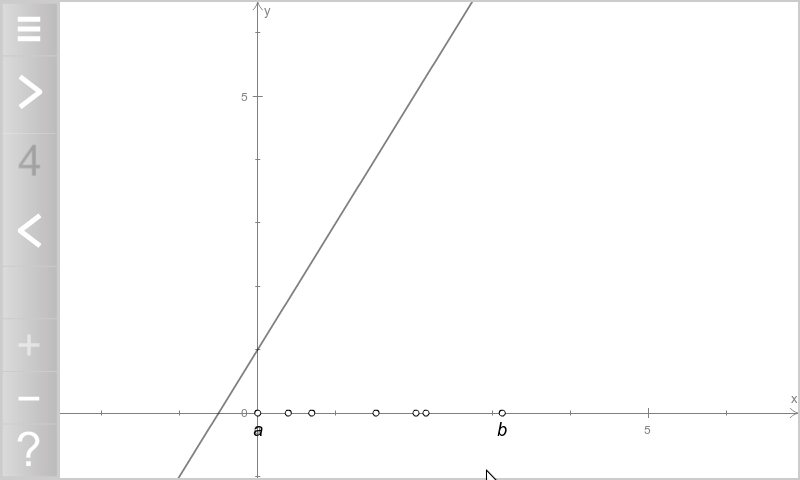
\includegraphics[width=0.5\textwidth]{particao.png}
	\caption{exemplo de partição do intervalo $[a,b] = [0,3]$. Note como os pontos $x_i$ da partição foram escolhidos de modo que a distância entre eles varia. Isso é importante para mostrar a arbitrariedade inerente à construção de uma soma de Riemann.}
	\label{fig:particao}
      \end{figure}

      \item Na tela 5, construa os elementos de área, isto é, os retângulos de base $\Delta x_i = x_{i+1} - x_i$ e altura $f(\xi_i)$, onde $\xi_i$ é um número \emph{arbitrário} do subintervalo $[x_i, x_{i+1}]$ e $i = 0,1,\ldots,n-1$. Note que a área do $i$-ésimo elemento de área é igual a $f(\xi_i)\Delta x_i$.
      
      Para criar um elemento de área no software, clique no gráfico de $f$ em algum $\xi_i \in [x_i,x_{i+1}]$. Ao fazer isso, aparecerá o símbolo $\times$ sobre o gráfico de $f$, destacando o ponto $\left(\xi_i, f(\xi_i)\right)$. Neste momento, pressione o botão $+$ (mais) ou a tecla \textit{p} para que o elemento de área (um retângulo) seja automaticamente desenhado na tela. Se você repetir esse procedimento para um $\xi_i$ diferente do mesmo subintervalo, um novo elemento de área será criado no lugar do anterior. Para remover um elemento de área, clique sobre ele e pressione o botão $-$ (menos) ou a tecla ``delete''.
      
      Repita o procedimento acima para cada subintervalo, \emph{sem se preocupar com o critério de escolha de $\xi_i$}, pois um dos objetivos desta atividade é que esse ajuste seja feito manualmente.
      
      \item Ainda na tela 5, com todos os elementos de área presentes, questione os alunos sobre se a área encontrada, por meio dos retângulos, é uma boa aproximação. Note que você pode comparar a área exata ($=12$), calculada no passo \ref{step:area}, com a soma das áreas dos elementos de área, que é exibida no canto superior direito da tela.
      
      \item Motive os alunos a melhorar a aproximação. Para isso, chame a atenção para o fato de que em cada subintervalo há áreas ``sobrando'' (à esquerda de $\xi_i$) e ``faltando'' (à direita), e que a escolha de $\xi_i$ é arbitrária. Espera-se que os alunos proponham escolher $\xi_i$ de modo que, em cada subintervalo, o excesso de área à esquerda compense a falta dela à direita.
      
      Para fazer isso com o software, mova o mouse pelo subintervalo enquanto pressiona a tecla \textit{p} várias vezes, reconstruindo assim o elemento de área para vários $\xi_i$. Faça isso até que, \textbf{visualmente}, o excesso de área à esquerda de $\xi_i$ compense a falta à direita.\footnote{\textbf{Dica:} ao clicar sobre um elemento de área, aparecem duas retas verticais, uma à esquerda e outra à direita dele, que podem servir de guias para avaliar as áreas que faltam e que sobram.} Neste caso, $f(\xi_i)$ será o \emph{valor médio} de $f$ no subintervalo $[x_i, x_{i+1}]$.
      
      \paragraph{Observação:} quando escolhemos os $\xi_i$ de modo que $f(\xi_i)$ seja mínimo em cada subintervalo $[x_i,x_{i+1}]$, ao somar os elementos de área obtemos a chamada ``soma inferior'', que subestima a área sob $f$. Por outro lado, quando escolhemos $\xi_i$ de modo $f(\xi_i)$ seja máximo, obtemos a ``soma superior'', na qual a área é superestimada.
      
      \item Ajuste cada um dos $\xi_i$ conforme o critério do passo anterior. No final, compare novamente a soma das áreas dos elementos de área, no canto superior direito da tela, com a área obtida com argumentos geométricos (passo \ref{step:area}).
      
      Avance para a tela 6, tomando o cuidado de verificar se a quantidade de elementos de área desenhados é igual à quantidade $n$ de subintervalos: apenas nesta condição o software permitirá avançar.
      
      \item Na tela 6 o software exibirá o gráfico da primitiva (ou anti-derivada) de $f$, a função $F$, sobreposta à construção realizada até aqui. Se quiser ver a expressão analítica dela, clique sobre $F$ para selecioná-la e pressione o botão ? (ajuda), no canto inferior esquerdo da tela. Nessa proposta, $F(x) = x^2/2 + x + C$, onde $C$ é a \emph{constante de integração}.
      
      \item Arraste $F$ para cima e para baixo, o que corresponde a variar $C$ (note que o valor da constante de integração varia conforme você faz isso: consulte o valor pressionando novamente o botão de ajuda, com a função $F$ selecionada). Argumente que essa ação não afeta a relação entre $f$ e $F$, isto é, $f = dF/dx$, pois a derivada de uma constante é nula.
      
      Essa etapa da atividade mostra que, ao integrar uma função, sua primitiva será, na verdade, uma família de funções, pois para cada valor de $C$, tem-se uma nova função.
      
      \item \label{step:C} Arraste $F$ para baixo, até que seu vértice aproxime-se de $y = -5$ (neste caso, $C \approx -4,7$). O intuito desse passo é apenas facilitar o passo seguinte.
      
      \item Obtenha o valor de $F(a)$: clique próximo do ponto $\left(a,F(a)\right)$ para destacá-lo no plano cartesiano, como ilustrado na figura \ref{fig:F(a)}. Em seguida, pressione o botão ? (ajuda) para ler o valor de $F(a)$ na janela de ajuda.
      
      \begin{figure}
	\begin{minipage}[t]{0.49\textwidth}
	  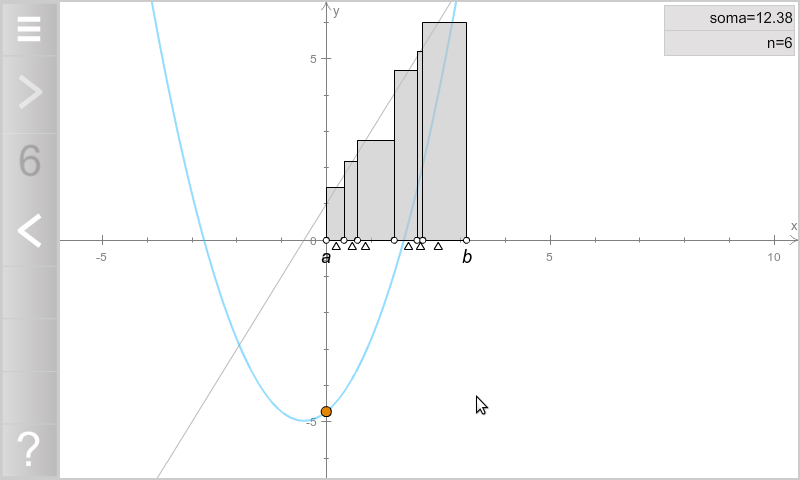
\includegraphics[width=\textwidth]{F(a).png}	  
	  \caption{selecione o ponto $\left(a,F(a)\right)$ e acesse a janela de ajuda para conhecer o valor de $F(a)$.}
	  \label{fig:F(a)}
	\end{minipage}
	\hfill
	\begin{minipage}[t]{0.49\textwidth}
	  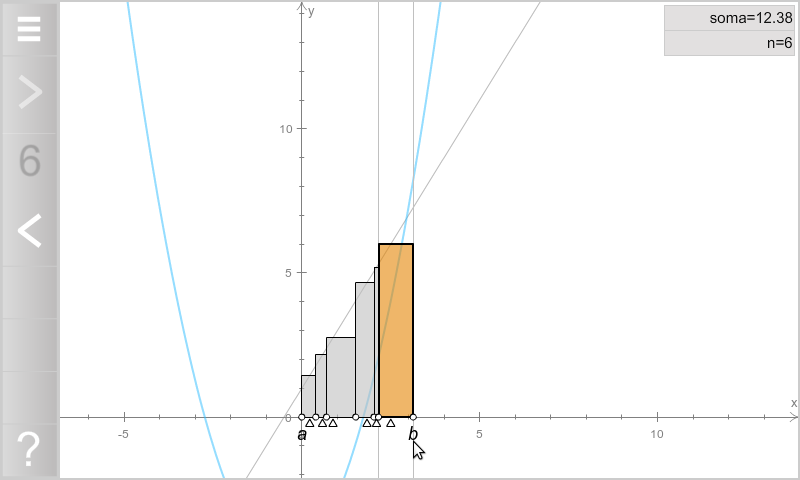
\includegraphics[width=\textwidth]{linhas-guia.png}
	  \caption{utilize as linhas-guia verticais para selecionar o ponto $\left(b,F(b)\right)$.}
	  \label{fig:linhas-guia}
	\end{minipage}	
      \end{figure}
      
      \item Obtenha o valor de $F(b)$, como no passo anterior.
      
      Em alguns casos pode ser difícil acertar o clique sobre $\left(b,F(b)\right)$.\footnote{Especialmente se você não fez $C \approx 4,7$, como instruido no passo \ref{step:C}.} Para simplificar essa tarefa, selecione o elemento de área mais à direita para que o software desenhe as linhas-guia verticais nas laterais dele (fig~\ref{fig:linhas-guia}). Deste modo, basta clicar sobre a intersecção da linha vertical mais à direita com $F$ para obter $F(b)$.
      
      \item Calcule $F(b) - F(a)$ e compare o resultado com os valores da soma de Riemann, no canto superior direito, e da área obtida com argumentos geométricos (passo \ref{step:area}). O resultado desses três procedimentos deve ser o mesmo, igual a (ou aproximadamente) 12. Esta é uma evidência do \emph{teorema fundamental do Cálculo}, a saber:
      \begin{equation}\label{eq:TFC}
       \text{Área sob $f$ em $[a,b]$} = \int_a^b f(x)\,dx = F(b) - F(a).
      \end{equation}
      
      É fundamental chamar a atenção dos alunos para os dois últimos procedimentos: no primeiro, aproximamos a área sob $f$ pela soma da área de $n$ retângulos (\emph{matemática discreta}); no segundo, utilizamos a anti-derivada $F$ para calcular $F(b) - F(a)$ (\emph{matemática contínua}). A equivalência entre esses dois resultados é o teorema fundamental do Cálculo, que nos permite obter a \emph{integral definida de $f$ em $[a,b]$} (a área sob $f$) sem efetuar a laboriosa soma de Riemann.
      
      \paragraph{Atenção:} este é um bom momento para distinguir a ``área sob $f$'' da ``integral de $f$''.
      Rigorosamente, a ``área sob $f$'' é de fato a área da \emph{região} delimitada por $x = a$, $x = b$, $y = 0$ e $y = f(x)$.
      Por exemplo, a \emph{integral} de $f(x) = x$ no intervalo $[1,-1]$ é igual a zero:
      \begin{equation*}
	\int_{1}^{-1} x\, dx = \left[\frac{x^2}{2}\right]_{1}^{-1} = 0,
      \end{equation*}
      mas a ``\emph{área} sob $f$'' nesse intervalo é igual a um:
      \begin{equation*}
	\left|\int_{1}^{-1}|x|\,dx\right| = \left|\int_{1}^{0}(-x)\, dx + \int_{0}^{-1}x\, dx\right| = 1.
      \end{equation*}
      
      Assim, embora a \emph{integral} possa ser positiva ou negativa, a \emph{área} só pode ser positiva.
      
      Note na última expressão que, para calcular a área, integramos $|x|$ ao invés de $x$, visando garantir que o integrando seja sempre positivo.
      Além disso, tomamos o módulo da integral para evitar o sinal negativo oriundo da orientação do intervalo de integração ($dx < 0$).
      
    \end{list}
    
    \section*{Parte 2}
    
      Nesta segunda parte, aplicaremos os dois conceitos explorados na parte anterior (soma de Riemann e teorema fundamental do Cálculo)
      para encontrar a integral de $f(x) = x^2$ no intervalo $[0,3]$. Note que não poderemos utilizar a Geometria Euclidiana Plana.
    
      \subsection*{Objetivos específicos}
  
      Ao final desta parte, espera-se que os alunos saibam:
      \begin{compactitem}
	\item explicar o significado dos termos \emph{soma inferior} e \emph{soma superior}.
	\item relacionar o aumento na quantidade de elementos de área com a melhoria na aproximação da área pela soma de Riemann.
      \end{compactitem}
      
      \subsection*{Roteiro}
           
      \begin{list}{\arabic{steps}.}{
	\setlength\leftmargin{0cm}%
	\setlength\itemindent\parindent%
	\setlength\listparindent{\parindent}%
        \setlength\labelwidth{1.3em}%
        \setlength\labelsep{0.7em}%        
        \refstepcounter{steps}%
        \usecounter{steps}%
      }
    
	\item calcular integral de $f$
	\item selecionar $f(x) = x^2$
	\item selecionar $[a,b] = [0,3]$
	\item selecionar ``soma inferior'' (``soma superior'')
	\item chamar a atenção para o erro ``para menos'' (``para mais'')
	\item aumentar/reduzir o número de elementos de área, chamando a atenção para a progressão da somatória, cada vez mais próxima da integral.
	\item No limite em que $n \to \infty$, abordar a transição do discreto para o contínuo.
    
      \end{list}
      
    \subsection*{Parte 3}
    
      Na parte final desta atividade os alunos replicarão o que foi exposto para outras funções simples.
    
    \subsection*{Objetivos específicos}
  
      Ao final desta parte, espera-se que os alunos saibam:
      \begin{compactitem}
	\item calcular uma integral simples pelo teorema fundamental do Cálculo.
	\item construir a soma de Riemann associada utilizando o recurso educacional interativo.
      \end{compactitem}
      
      \begin{list}{\arabic{steps}.}{
	\setlength\leftmargin{0cm}%
	\setlength\itemindent\parindent%
	\setlength\listparindent{\parindent}%
        \setlength\labelwidth{1.3em}%
        \setlength\labelsep{0.7em}%        
        \refstepcounter{steps}%
        \usecounter{steps}%
      }
      
	\item separar a classe em grupos de 5 alunos
	\item atribuir uma função da lista do recurso educacional interativo para cada grupo (informar também a primitiva)\footnote{Isto é importante, pois
	ainda não abordamos as propriedades da integral, de modo que os alunos não sabem como tratar soma de funções, multiplicação por constante etc.}
	\item instruir cada grupo a efetuar a integração
	\item chamar, um grupo por vez, para o computador do professor, para efetur a construção da soma de Riemann (fica a critério dos alunos escolher o
	tipo de soma que quiser).
	\item o professor escreve no quadro uma tabela contendo os grupos nas linhas e, nas colunas, o resultado da integração via teorema fundamental do
	Cálculo e via soma de Riemann. Cada grupo fica responsável por preencher sua linha da tabela. Enquanto um grupo vai na frente construir a somar
	de Riemann, os demais fazem o cálculo pelo teorema fundamental, e vice-versa.
	\item no final da atividade, que deve demorar aproximadamente 5 minutos por grupo, a tabela evidenciará a equivalência entre os resultados.
	Caso não dê tempo de todos os grupos participarem, proponha que eles terminem o exercício por conta própria, acessando o recurso educacional 
	por meio do AVA.
      
      \end{list}
    
  \section*{Nomenclatura}
    \begin{compactitem}
      \item Uma \emph{partição} $P$ do intervalo de integração é um conjunto de pontos $x_i$ sobre o eixo das abscissas que dividem o intervalo de integração em $n$ subintervalos, com $i = 0, 1, \ldots, n$. Os limites inferior (representado por $a$) e superior ($b$) compõem o primeiro e último desses pontos, respectivamente. Ou seja, $P = \{x_0 = a, x_1, \ldots, x_n = b\}$.
      
      \item $x_i$ é o $i$-ésimo ponto da partição do interalo $[a,b]$.
      
      \item $\Delta x_i = x_{i+1} - x_i$ é a amplitude do $i$-ésimo subintervalo de integração.
      
      \item $\Delta a_i = f(\xi_i) \Delta x_i$ é a área do $i$-ésimo \emph{elemento de área}, um retângulo de base $\Delta x_i$ e altura $f(\xi_i)$, onde $\xi_i$ é um ponto qualquer do subintervalo de integração $[x_i, x_{i + 1}]$.

      \item \emph{Teorema do valor médio} para integrais (TVM): se $f$ for uma função contínua em $[a,b]$, então existirá ao menos um $\xi \in [a,b]$ tal que $\int_a^b f(x)\,dx = (b-a) f(\xi)$, onde $f(\xi)$ é o valor médio de $f$ em $[a,b]$.

      \item Uma \emph{primitiva}, ou \emph{anti-derivada} da função $f$ é a função $F$ tal que $f = \frac{dF}{dx} = \frac{d}{dx}\left(F + C\right)$, onde $C$ é a \emph{constante de integração}.

      \item A \emph{soma de Riemann} $S_n$ é a soma de todos os elementos de área. Ou seja, $S_n = \sum_{i=1}^{n} f(\xi_i) \Delta x_i$.

      \item A \emph{integral de Riemann} é o limite da soma de Riemann quando $n$ tende ao infinito. Ou seja, $I = \lim_{n \to \infty} S_n$. Neste limite, o critério de escolha de $\xi_i$ (soma superior, soma inferior ou personalizada, como usamos nesta proposta) é irrelevante para o resultado: $I = \int_a^b f(x)\, dx$.

      \item O \emph{teorema fundamental do Cálculo} diz que, se $f$ for contínua em $[a,b]$, então $\int_a^b f(x)\,dx = F(b) - F(a)$, onde $F$ é qualquer anti-derivada de $f$.
    \end{compactitem}

  \section*{Créditos}
  
  O recurso educacional interativo utilizado nesta proposta foi inicialmente desenvolvido para a disciplina ``Fundamentos de Matemática'' (\href{https://uspdigital.usp.br/jupiterweb/obterDisciplina?sgldis=plc0001&nomdis=}{PLC0001}) do curso de graduação semi-presencial em Licenciatura em Ciências do convênio USP/Univesp (Universidade Virtual do Estado de São Paulo), numa parceria dos autores com o Centro de Ensino e Pesquisa Aplicada (\href{http://cepa.if.usp.br}{CEPA}) da USP.


\end{document}
